\subsection{Predictors and probabilistic model}
\label{sec:methods-models}


After deriving the \emph{OCO-2-relative} anomaly ($\Delta \mathrm{X_{CO2}^{B11}}$) in Sect.\ref{sec:method-cld_dist_xco2_anom} and the photon path-length features in Sect.\ref{sec:methods_photon_path}, we build deep-ensemble multilayer perceptron (\emph{DE-MLP}) models to predict and correct $\Delta \mathrm{X_{CO2}^{B11}}$. Separate models are trained for land and ocean footprints. We also compare the model performance with ridge linear regression (\emph{Ridge}) and gradient-boosted decision trees (\emph{XGBoost}) models.

We use $\Delta \mathrm{X_{CO2}^{B11}}$ as the truth for training, and features from photon path-length fitting (Sect.\ref{sec:methods_photon_path}), full-physics retrieved variables in the lite files, EOFs of temperature, water vapor, and \ce{CO2} profiles, geometry and L1B diagnostics, contamination indicators, and a one-hot-encoded footprint identifier. Details of the variables used as predictors for ocean and land footprints are given in Table~\ref{tab:predictors}, which also shows the subgroups of variables used in the subgroup importance analysis. We compare the performance of the full predictor set against sets that (1) exclude $\mathrm{X_{CO2,}^{raw}}-\mathrm{X_{CO2}^{prior}}$, (2) exclude the photon path-length features, (3) exclude the contamination indicators, (4) exclude both $\mathrm{X_{CO2}^{raw}}-\mathrm{X_{CO2}^{prior}}$ and the photon path-length features, and (5) exclude both $\mathrm{X_{CO2,}^{raw}}-\mathrm{X_{CO2}^{prior}}$ and the contamination indicators. All features are normalized and standardized based on the training set before the training and prediction processes.

We compare the \emph{Ridge}, \emph{XGBoost}, and \emph{DE-MLP} models with the
full feature set. \emph{Ridge} is an $\ell_2$-regularized linear regression with
its penalty selected on the calibration subset. \emph{XGBoost} uses 500 boosting
rounds with a maximum tree depth of 6. The \emph{DE-MLP} is an ensemble of five
Gaussian-head MLPs; each member has two hidden layers (64 and 32 units) with
layer normalization, ReLU activation, and 10\% dropout, and a two-output head
predicting the mean anomaly $\mu_{m,i}$ and its log-variance
(Fig.~\ref{fig:DE_structure}). The members are trained by minimizing the
$\beta$-NLL loss of \citet{seitzer2022pitfalls} ($\beta = 0.5$), a
variance-weighted Gaussian negative log-likelihood that keeps the mean well
fitted in the high-variance near-cloud regime; the loss and the full training
configuration are given in Appendix~\ref{app:model}. The five members differ
only in their random seed, and their Gaussian mixture yields the ensemble mean
$\mu^{*}_i$—the point correction applied to each footprint—together with a
predictive variance that separates aleatoric and epistemic components
(Appendix~\ref{app:model}). The calibration subset is used to recalibrate the
Mondrian conformal intervals, which are binned by predicted-anomaly deciles.

The nearest cloud distance is never used as a model predictor. It is only used in the construction of the training target (Sect.~\ref{sec:method-cld_dist_xco2_anom}) and the evaluation stratification. The correction is applied one footprint at a time from per-sounding L2 Lite quantities, so the model performs no aggregation over neighboring soundings at inference.\footnote{A few contamination indicators (the \texttt{h\_continuum}
band diagnostics) are per-sounding preprocessor values that internally summarize local continuum-radiance variability across adjacent soundings; they are still supplied as single-sounding inputs and require no access to neighboring footprints at deployment.}


% We compare the performance of the \emph{Ridge}, \emph{XGBoost}, and \emph{DE-MLP} models with the full feature set. The \emph{Ridge} model represents a regularized linear multiple-variable regression, with its regularization strength selected on the calibration subset. The \emph{XGBoost} model is set to use 500 boosting rounds (trees) and a maximum tree depth of 6. The \emph{DE-MLP} model consists of five Gaussian-head MLP members. Each member contains three layers. The first layer has 64 perceptrons connecting to the input features, followed by a normalization layer, a ReLU activation, and a 10\% dropout layer. The second layer has 32 perceptrons connecting to the previous output, also followed by a normalization layer, a ReLU activation, and a 10\% dropout layer. The third layer has two perceptrons with linear activation to predict the output anomaly $\mu_{\mathrm{m}-i}$ and the uncertainty $\log{\sigma_{\mathrm{m}-i}^2}$. Each member $m$ is a Gaussian-head MLP that, for footprint $i$, outputs a
% predicted mean $\mu_{m,i}$ and a raw second output that is clamped to
% $[-10, 10]$ and interpreted as the log-variance
% $s_{m,i} = \log\sigma_{m,i}^{2}$, giving a per-footprint predictive variance
% $\sigma_{m,i}^{2} = \exp(s_{m,i})$. Writing the target as
% $y_i \equiv \Delta \mathrm{X_{CO2,\,i}^{B11}}$, the standard Gaussian negative
% log-likelihood of one footprint is, up to an additive constant,
% %
% \begin{equation}
%   \ell^{\mathrm{NLL}}_{m,i}
%   = \frac{1}{2}\left[\,s_{m,i}
%   + \frac{(y_i-\mu_{m,i})^{2}}{\sigma_{m,i}^{2}}\,\right].
%   \label{eq:gauss-nll}
% \end{equation}
% %
% Because this loss down-weights high-variance footprints, the mean is poorly
% fitted exactly in the near-cloud regime where $\sigma_{m,i}^{2}$ is large. We
% therefore train the members with the $\beta$-NLL loss of
% \citet{seitzer2022pitfalls}, which multiplies each footprint's NLL by a
% stop-gradient function of its own predicted variance,
% %
% \begin{equation}
%   \ell^{\beta\text{-}\mathrm{NLL}}_{m,i}
%   = \bigl\lfloor\sigma_{m,i}^{2}\bigr\rfloor_{\mathrm{sg}}^{\,\beta}\;
%   \ell^{\mathrm{NLL}}_{m,i},
%   \qquad \beta = 0.5,
%   \label{eq:beta-nll}
% \end{equation}
% %
% where $\lfloor\cdot\rfloor_{\mathrm{sg}}$ denotes a stop-gradient (the weight
% is treated as a constant during backpropagation). Here $\beta = 0$ recovers the
% plain NLL of Eq.~\eqref{eq:gauss-nll} and $\beta = 1$ recovers a mean-squared-error
% weighting of the mean; the production choice $\beta = 0.5$ restores the
% mean-fitting gradient in the high-variance near-cloud footprints while keeping
% a calibrated variance. The member loss is the average of
% Eq.~\eqref{eq:beta-nll} over the training footprints.

% Each member is optimized with AdamW (learning rate $10^{-3}$, weight decay
% $10^{-4}$) under a one-cycle learning-rate schedule with gradient-norm clipping
% at $1.0$, a batch size of $4096$, and up to $500$ epochs. Training is stopped
% early on the held-out calibration block (patience of $50$ epochs), and the
% checkpoint with the lowest calibration loss is kept; the calibration block is
% carved from the training dates and never overlaps the held-out fold or the
% validation references. The five members differ only in their random seed
% (member $m$ uses seed $s_0 + m$), so their predictions decorrelate and the
% ensemble spread provides the epistemic uncertainty. The per-member means and
% variances are combined as a Gaussian mixture,
% %
% \begin{equation}
%   \mu^{*}_i = \frac{1}{M}\sum_{m=1}^{M}\mu_{m,i},
%   \qquad
%   \sigma^{*2}_i
%   = \underbrace{\frac{1}{M}\sum_{m=1}^{M}\sigma_{m,i}^{2}}_{\text{aleatoric}}
%   + \underbrace{\frac{1}{M}\sum_{m=1}^{M}\mu_{m,i}^{2} - \mu^{*2}_i}_{\text{epistemic}},
%   \label{eq:mixture}
% \end{equation}
% %
% which is the law of total variance: the first term is the mean aleatoric
% variance predicted by the heads and the second is the between-member (epistemic)
% variance. The ensemble mean $\mu^{*}_i$ is the point correction applied to each
% footprint. The structure of the \emph{DE-MLP} model is illustrated in Fig.~\ref{fig:DE_structure}. The calibration subset is used to recalibrate the Mondrian conformal bins, which are defined by predicted-anomaly deciles. Note that cloud distance is never used as a model predictor; the nearest-cloud
% distance enters only the construction of the training target
% (Sect.~\ref{sec:method-cld_dist_xco2_anom}) and the evaluation stratification.
% The correction is applied one footprint at a time, and every predictor is a
% per-sounding quantity read directly from the OCO-2 L2 Lite product, so the model
% performs no aggregation over neighboring soundings at inference. A few
% contamination indicators (the \texttt{h\_continuum} band diagnostics) are
% per-sounding preprocessor values that internally summarize the local
% continuum-radiance variability across adjacent soundings; they are nonetheless
% supplied to the model as single-sounding inputs and require no access to
% neighboring footprints when the correction is deployed.




%
\begin{figure}[t]
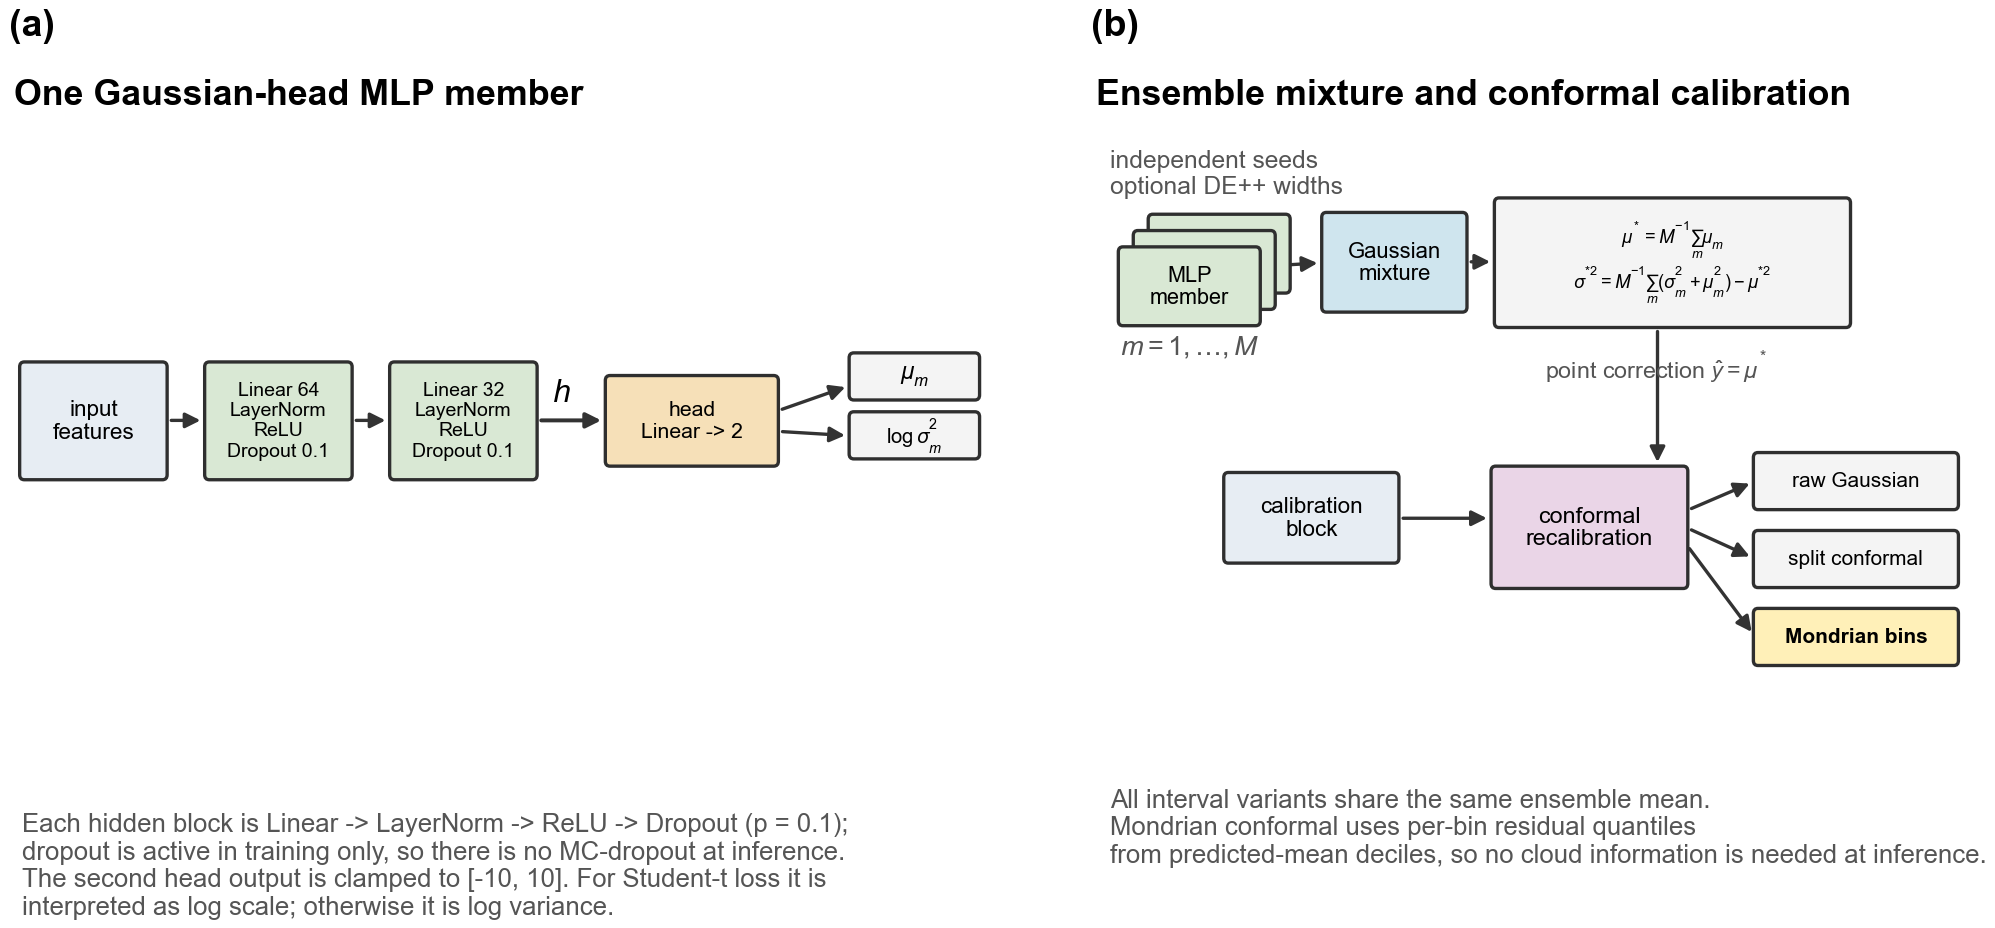
\includegraphics[width=\textwidth]{figures/fig02_deep_ensemble_architecture.png}
\caption{Per-surface probabilistic correction model. (a) One Gaussian-head MLP member (64→32 hidden units; layer normalization and dropout 0.1; $\mu$, $\log{\sigma^2}$ heads; $\beta$-NLL loss, $\beta$ = 0.5). (b) M = 5 members per fold pooled as a Gaussian mixture, followed by split and Mondrian conformal calibration of the 90 \% intervals. All inputs are per-sounding L2 Lite quantities: cloud distance enters only label construction and evaluation — never the model input — so the correction runs footprint-by-footprint with no imager and no along-track context at inference.}
\label{fig:DE_structure}
\end{figure}
%

